\section{Evaluation}
\subsection{Properties of the dark current}
We cooled the CCD-Chip\footnote[1]{This is a highly sensitive photon detector which operates by letting incoming photons excite the electrons of the picture elements (pixels) represente by metal oxide semiconductor capacitors on a silicon substrate into the respective conduction band, where these electrons get converted into a voltage which then again is converted into a digital signal by an analogue to digital converter.} using liquid nitrogen in order to reduce the dark current produced by thermally excited electrons within the CCD-chip, which deteriorates the sensitivity of our camera and decreases the dynamical range of our system. While cooling down the detector we repetitively measure the dark current by taking exposures of 30 seconds with closed shutter. After all images are taken, we correct each of them for their bias \footnote[2]{which we determine as the median count value in the overscan region (only contains the positive offset/bias applied to all detector pixels. This offset is required as the analog-digital-converter can only handle positive pixel values and due to fluctuations or bad behaving pixels negative values might otherwise occur) containing only the offset voltage, the bias}. We are now able to determine the dark current as the median of the bias-subtracted images:

\begin{figure}[h]
	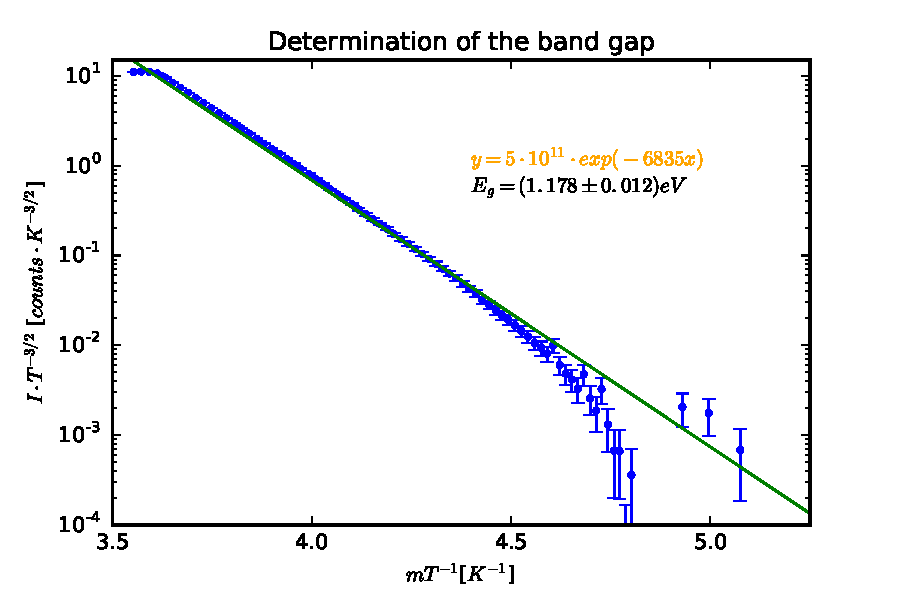
\includegraphics[width=100mm]{diag2}
	\centering
	\caption{ \itshape Band gap of the silicon semiconductor based CCD }
	\label{fig:Abbildung 2}
\end{figure}
\noindent
By fitting function (14) from the manual, this is
\[I = \mathrm{const.}\cdot T^{3/2}\cdot \exp{-\frac{E_g}{2k_bT}}\]

 to the data as shown in figure \ref{fig:Abbildung 2} we determine the band gap of the detector to be $E_g = \left(1.178\pm0.012\right)\mathrm{eV}$. Thus, our measured value deviates from the literature value non significantly of $E_{g,lit,Si}=1.5 \mathrm{eV}$ at $302 K$ (compare \url{https://en.wikipedia.org/wiki/Band_gap}, accessed 11/04/18, 13:53) by $2.3\sigma$.\\
As described above we had to subtract the bias from every image individually in order to calculate the median dark current. The bias ranges between 1320 counts for higher temperatures ($~ -16.7 ^{°}C$) and 1336 counts for low temperatures (~$-104.5^{°}C$), slightly increasing roughly linearly with decreasing temperature. We therefore had to corect every image individually for its bias.


\subsection{Flat-Field correction}
The raw images take with the CCD-camera exhibit both small- and large-scale variations that we have to get rid off in order to be able to compare brightness in different areas on the camera.  We took five dome-flats (we used a white blanket illuminated by an orange lamp) for the I- and V-filter (Johnson system). Due to the different intensity of our light source in different filters, we had to adjust the exposuretime for both filters.
\begin{figure}[h]
	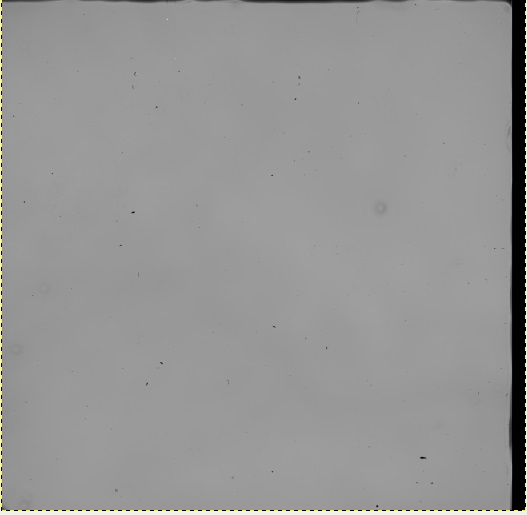
\includegraphics[width=70mm]{flat}
	
\includegraphics[width=70mm]{flat_norm}
	\centering
	\caption{ \itshape From left to right: individual flat-field, corrected flat-field }
	\label{fig:Abbildung 3}
\end{figure}
\noindent
 After the flat fields were taken, we subtracted the bias from each image individually, as above. Then, we combined the five images (for both filters separately) to two masterflat-fields by taking the median (We use the median for combing the images, because if we used the mean for example, very high or low pixel values, due to cosmic rays or in general bad pixels, would distort the result much more than when taking the median) pixel by pixel. In a last step, we normalised each of these masterflat-fields by dividing every of its pixel values by the median taken over all of its pixel values.
 The master-flat-field has to be normalised, because in the end we do not want to change the overall intensity of the science frame.In order to see the effect of a flat-field correction, we corrected one of the indiviual flat-field images by dividing it by the normalised master-flat-field, this can be seen in figure \ref{fig:Abbildung 3}
As we expect, the flat-field corrected flat-field image has more or less the same pixel value in every pixel, making it look like the flat surface that we want it to look like. On the right side of each picture we see the overscan region as explained above.\\

\begin{figure}[h]
	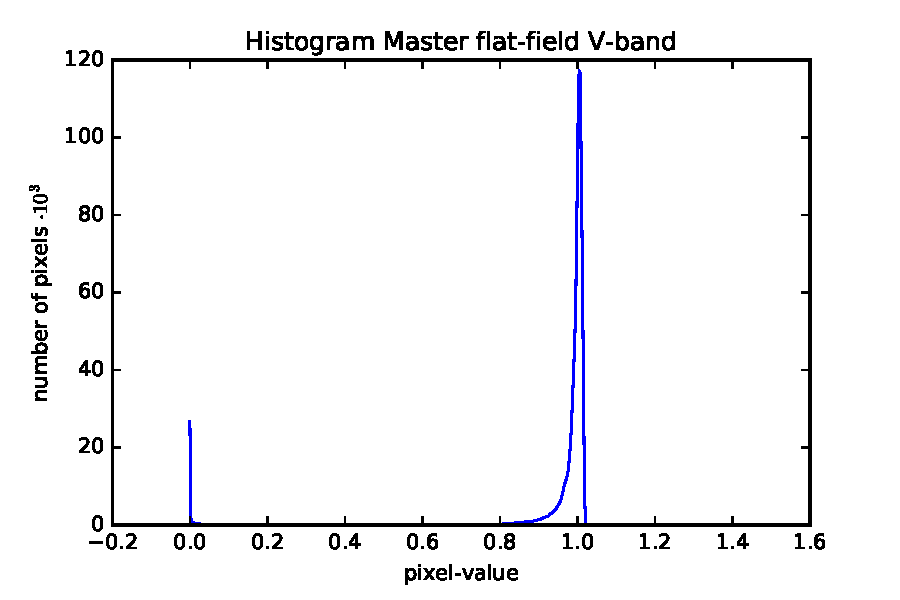
\includegraphics[width=70mm]{histogram_V}
	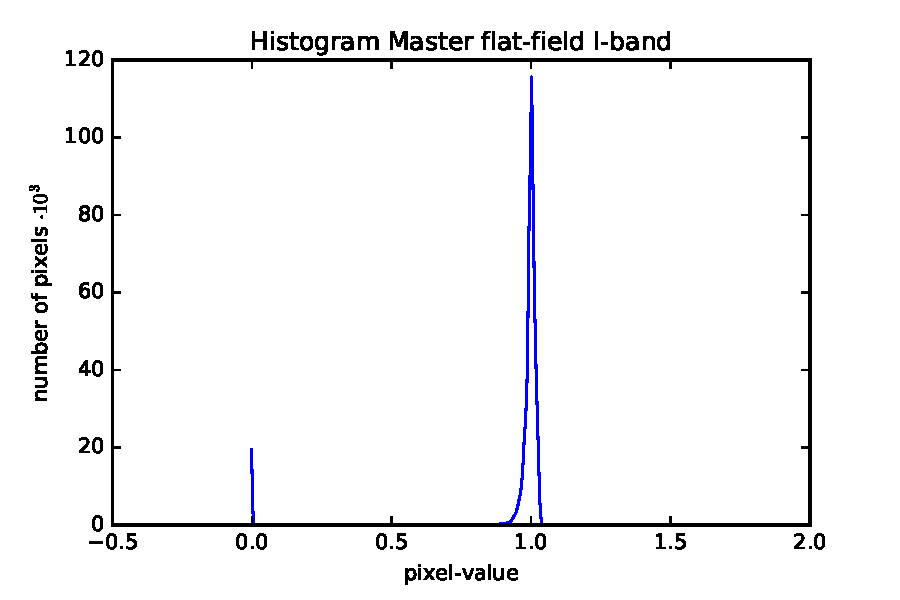
\includegraphics[width=70mm]{histogram_I}
	\centering
	\caption{ \itshape Left :Visual Johnson Filter centered around V = 551 nm, Right:  Infrared Johnson filter }
	\label{fig:Abbildung 4}
\end{figure}
\noindent
If we have a look at the histogram of our master flatfields (compare figure \ref{fig:Abbildung 4}) we notice that, just as we expect, most of the pixels have a value close to 1. The smaller peak around 0 results from the pixels in the overscan region: As the pixels in this region contain only the bias value, which is then subtracted from the image, these pixels have a value close to zero. This value gets even smaller during normalisation as they are divided by the overall mean of the picture. This explains why there are approximately 25.000 pixels with a value close to zero while there are around 100.000 pixels with values close to 1 (consider that the sensor physically has $1024 \times 1024$ pixels and adds another 26 columns (1024 pixels each) representing the overscan region in the interval $x\in \left[1023,1049\right]$ and $y\in \left[0,1024\right]$). 



\subsection{Linearity and dynamical range of the CCD}
In this part of the experiment we want to quantify the efficiency of the detector and its limitations by examining its linearity and dynamical range. To examine the linearity of the camera, we take again pictures of our flat surface but this time with varying exposure times. This is done for the I- and V-filter. We perforemd a bias- and flat-field correction on the resulting pictures. Then, we calculated the median and standard deviation of each image. Plotting these values of the exposure times results in figure \ref{fig:Abbildung 6}.
\begin{figure}[h]
	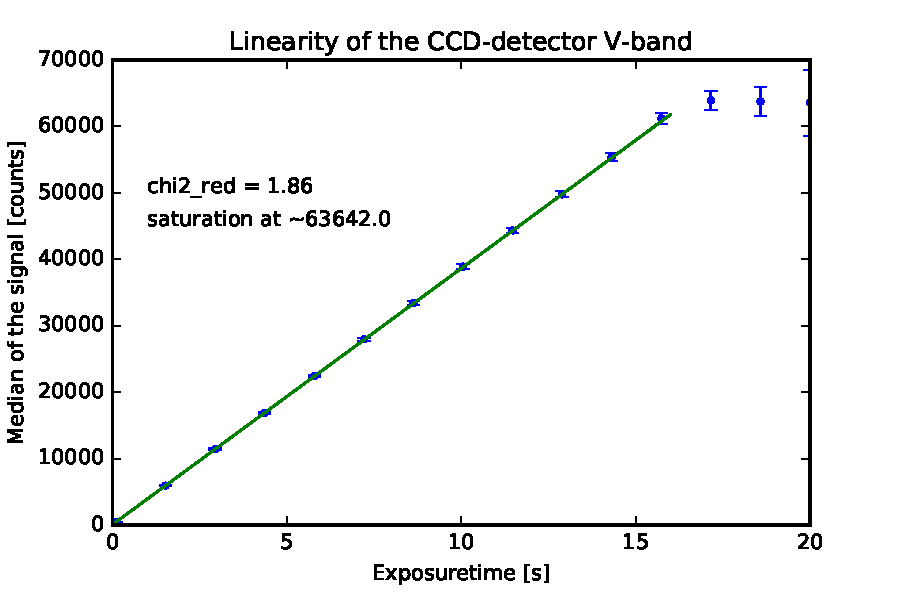
\includegraphics[width=70mm]{liniarity_V}
	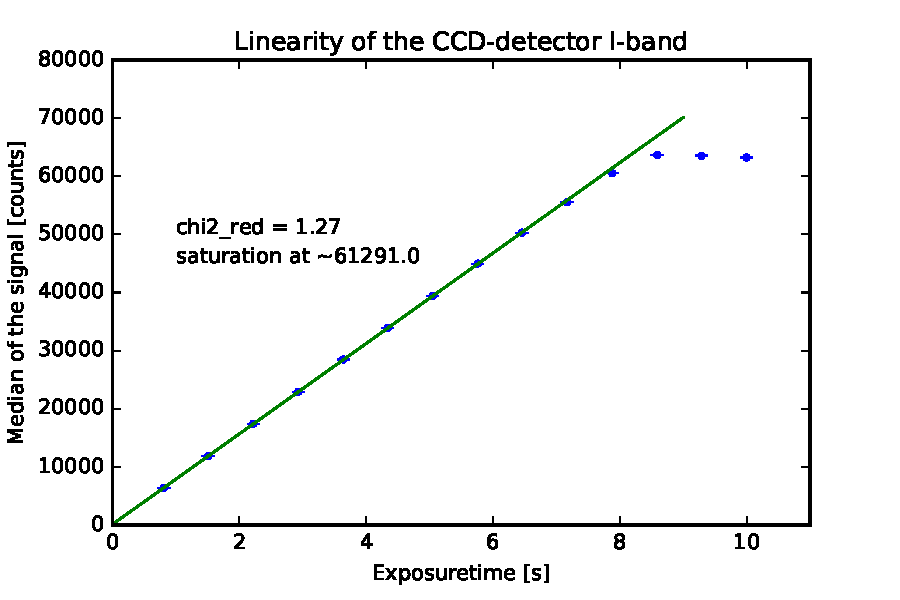
\includegraphics[width=70mm]{liniarity_I}
	\centering
	\caption{ \itshape From left to right: Linear relation of flux and integration time in the visual Johnson filter, linear relation of flux and integration time in the infrared Johnson filter  }
	\label{fig:Abbildung 5}


\end{figure}
\noindent
We notice, that the dependency is linear (as expected) up to a certain integration time where the detector is saturated. From the plots we see that saturations sets in at around $63.000$ counts.  In order to quantify the deviation from a linear dependence, a linear function has been fitted to the regime before saturations sets in. Thus, we can confirm tha the CCD detector is linear up to an illumination corresponding to pixel values of around $63.000$ counts. We furthermore observe that the fit is quite good, which is only due to us leaving out the last two values with highest illumination. We chose to do this as the pixels of the CCD are saturated at this point, such that the two datapoints of highest illumination are outside of the linearity range for both filters.


\subsection{Sensitivity of the detector and noise properties}


In order to remove the effect of PRNU, we took ten pairs of flat-field images in the I-filter with varying exposure times.

\subsubsection{4.5.3.1 Find and discuss the photon noise, the read-out noise, and the PRNU noise for one flat image. Which noise dominates? Explain}
\label{sec:5}
We averaged over one pair of images in order to obtain one value per exposure time. The read-out noise of the gate amplifier was obtained by taking the standard deviation of the overscan region.
We furthermore subtracted the pairs of images from each each other and then determined the noise and signal of the difference image in the chosen homogeneously illuminated region $x\in \left[308,672\right]$ and $y\in \left[344,739\right]$.
Two images with the same exposure time should approximately contain the same PRNU noise, it describes how uniformly distributed the pixel response is. We therefore computed the PRNU noise via the difference noise and the total noise measured in the same area of one image pair like :
\begin{equation}
\label{eq:1}
	\sigma_{PRNU,d} = |\sigma_{tot,d}-\sigma_{diff,d}|
\end{equation}
\noindent
 The photon noise, which describes the variance of the pixel-to-pixel fluctuations in a uniformly illuminated are (the one chosen above), is obtained via equation (21) of the manual through the total, read-out and PRNU noise by
 \begin{equation}
 \label{eq:2}
 	\sigma_{e,d}=	\sqrt{|\sigma_{tot,d}^{2}-\sigma_{PRNU,d}^{2}-\sigma_{r,d}^{2}|}
 \end{equation}
 We find in total
 \begin{align*}
	 \sigma_{e,d} &= 214.1 \\
	 \sigma_{r,d} &= 214.7 \\
	 \sigma_{PRNU,d} &= 7.5 
 \end{align*}
Altogether we find the PRNU noise to be clearly subdominant w.r.t. the read-out and the photon-noise. We did this calculation for the image pair with the shortest exposure time, thus low signal count. We expect the PRNU noise to rise strongly with rising signal count. We furthermore expect the photon-noise to fall off for higher signal count values as it is poissonianly distributed and directly depends on the gain, but has a different flux dependence than the read-out noise.\\
We furthermore find the characteristic PRNU factor $f$ via equation 
\[\sigma_{PRNU,d} = f \cdot 10000 = \sigma_{e,d}\]  
to be either $f_PRNU = 0.02$ or $f_e = 0.01$, where the subscript indicates form which noise it was computed.
The PRNU factor was given by the manual to be $f=0.01$, such that the value obtained from the photon noise fits better (omitting errors here). We expect the PRNU factor obtained from the PRNU noise to be more precise when we include all the images in the later section, as it is non-stochastic. Choosing a more homogeneously illuminated area to extract the total and difference noise from would probably result in the photon noise overall dominating the PRNU and read-out noise. That we measured the contrary to be true simply shows that the precision of our instruments and the data reduction via flat-field and bias correction where not optimal.\\


\subsubsection{4.5.3.2 Plot the variance of the signal versus the signal itself for all measurements with increasing exposure times in the I-filter and extract the elextron sensitivity $\kappa$ using eq. 23. Explain what this plot means}
 
  Then, we plotted the variance of the signal versus the measured signal itself, compare figure \ref{fig:Abbildung 8}. We fitted equation (23) from the function to manual in the rearranged form 
  \begin{equation}
  	\left[\sigma_{diff,d}^{2}-\sigma_{r,d}^{2}\right] = \frac{1}{\kappa} \cdot N_{e,d}
  \end{equation}  
  to the data in order to determine $\kappa$. 
\begin{figure}[h]
	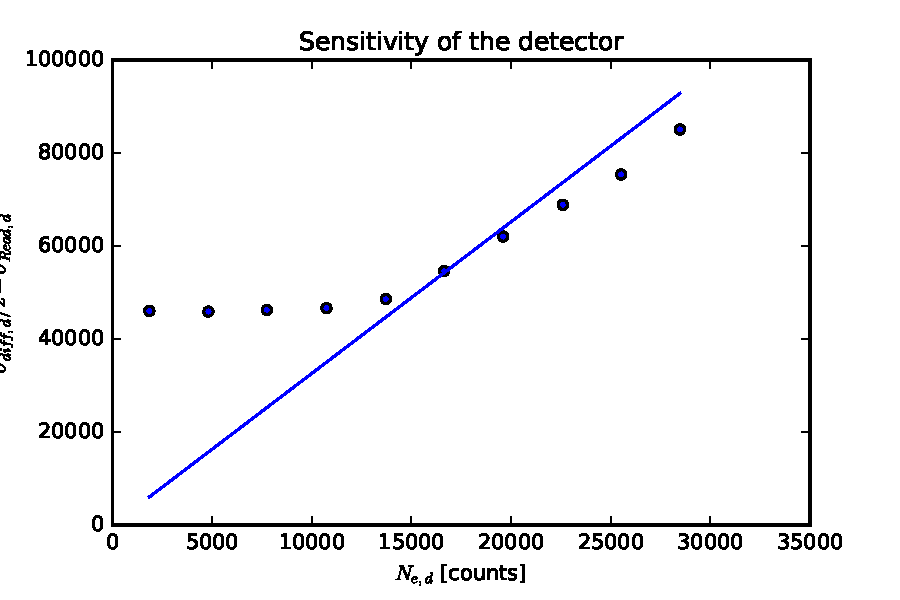
\includegraphics[width=100mm]{sensitivity}
	\centering
	\caption{ \itshape CCD gain  }
	\label{fig:Abbildung 8}
\end{figure}
\noindent
From the fit we obtained 
\[\kappa _{fit} = 0.31 \pm 0.34 \]
\noindent
with an enormous error, which is due to image pairs with low counts, thus low exposure times, not following the equation very well.
This plot therefore shows us, that the detector operates very well as predicted theoretically in a range of 
$10000-30000$ counts, this means that the signal processing works very well in this range, as the number of excited electrons per unit of the analogue digital converter, the gain $\kappa$, translates sensitively to the number of detected photons in this range.

\subsubsection{4.5.3.3 Calculate the electron sensitivity $\kappa$ using eq. (19) and explain discrepancies with the previous method. Do the calculation for just one image with average counts ~30000 ADU}

As described in section \ref{sec:5} we averaged over the pairs of images with same exposure time to obtain one value per exposure time. The read-out noise was again obtained as the standard deviation of the signal from the overscan region, the PRNU noise was determined by equation \ref{eq:1} and the photon noise was obtained by equation \ref{eq:2}. The electron sensitivity was then determined by equation (19) from the manual with a quantum efficiency of $100 \%$, as instructed by the manual by:
\begin{equation}
	\kappa_{calc} = \frac{N_{e,d}}{\sigma_{e,d}^{2}}
\end{equation}
\noindent
The values for all images are given in the attached python notebook. From this we extracted the electron sensitivity for one image with ~30000 counts to be 
\[\kappa_{calc} =  0.54 \pm 0.17\]
\noindent
where the error was obtained via the standard deviation of the different electron sensitivies, since the raw data values do not contain an error themselves. Comparing with the previous section we find that the electron sensitivity obtained from the fit and from the theoretical calculation differ differ non-significantly by $0.61 \sigma$ due to the enormous error for both values, which in turn is due to the high statistical error (standard deviation) as calculated from the chosen region.\\
From the overall data obtained here we again calculated the PRNU factor as above and found the different values via mean or median for all exposure times equally to be $f_{PRNU}=0.01$ and $f_e = 0.02$, such that the PRNU factor obtained from the whole data set by the PRNU noise is indeed comparable to the one given in the manual, as predicted above.

\subsection{Color Magnitude Diagram}
In this part of the experiment we will compute a Colour Magnitude diagram the globular cluster BS90 in order to estimate its age, distance and metallicity. To compute the CMD we use observations conducted in the I- and V-band by the Hubble Space Telescope.\\
\begin{figure}[h]
	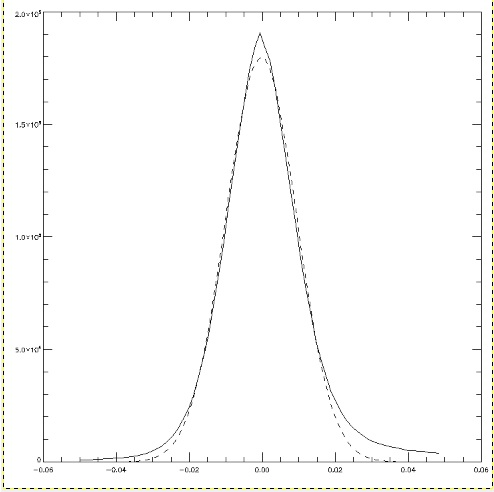
\includegraphics[width=70mm]{Inoise2}
	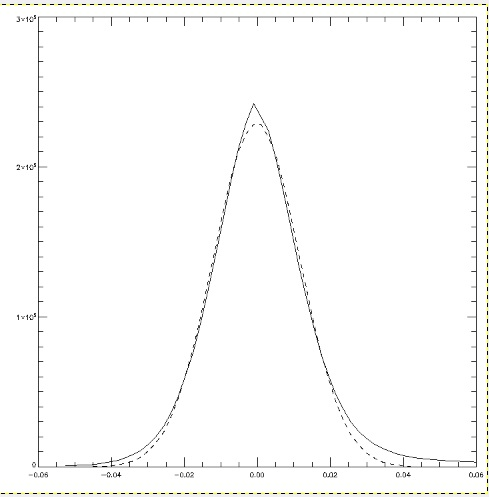
\includegraphics[width=70mm]{Vnoise}
	\centering
	\caption{ \itshape From left to right: Noise in the I band, Noise in the V band}
	\label{fig:Abbildung 9}
\end{figure}
\noindent
In a first step we had to determine the zeropoints for both filters in order to calibrate the instrument magnitude. We did this by determining the counts of ten different stars and relating them to the given Hubble instrumental magnitudes. Using equation (24) of the manual we individually determined the zeropoints. Their medians were found to be\\ 
\[zeropoint_V = 25.19 \pm 0.15 \qquad zeropoint_I = 24.97 \pm 0.26\]
\noindent
The error was estimated by the standard deviation via the formula (compare \url{http://davidmlane.com/hyperstat/A106993.html}):
\[\sigma_{median} \approx 1.253\frac{ \sigma_{stdev}}{\sqrt{N}}\]
To perform the photometric measurements, we use the software STARFINDER. To be able to identify the stars in the picture and to correctly determine their brightnesses, STARFINDER needs to compute the underlying noise first. The results can be found in figure \ref{fig:Abbildung 9}, where we observe that the noise count of the V-band is slightly higher but still comparable to the noise in the I-band.

Afterwards, we use STARFINDER to define a point-spread function from our images. This was very difficult to do especially for the I-band, as the precision within which one could select the stars to be considered was not very high. Due to us not being able to find an adequate PSF for the I band we used the produce of another group, who acquired said PSF a few weeks prior to us performing this experiment. Once this was done, we let the program identify all the magnitudes of the stars in the images. After cross-matching the outputs for both filters and adjusting the instrumental magnitudes using the zeropoints mentioned above, we can plout our CMD, compare figure \ref{fig:Abbildung 11}.
\begin{figure}[h]
	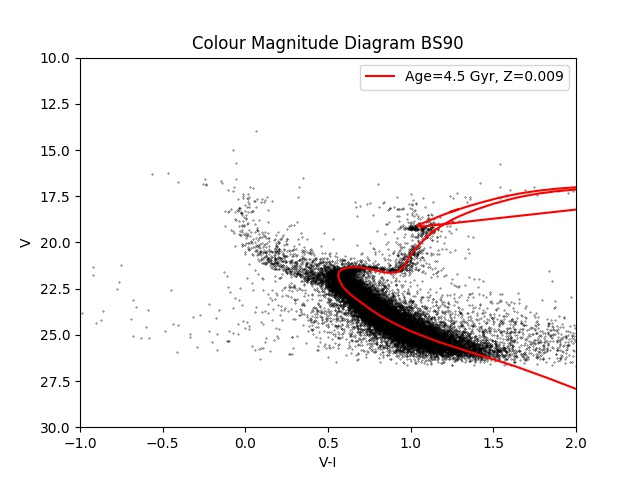
\includegraphics[width=100mm]{CMD}
	\centering
	\caption{ \itshape Color magnitude diagram for the BS90 cluster}
	\label{fig:Abbildung 11}
\end{figure}
\noindent
Using a $Y^{2}$ Isochrone plotting routine provided, we adjusted the parameters to get the best fitting isochrone for the main sequence of BS90. Age determination of globular clusters proceeds by adapting simulated stellar-evolution tracks to the Hertzsprung-Russel diagram (in this case CMD) of the given globular cluster and assign the age of the best-fitting stellar-evolution model (Isochrone) to the cluster, these show the displacement of stars of defined mass in the plane of the colour magnitude
diagram during their lifetime. Theoretical curves representing the position of the
stars of a stellar population of the same age can be calculated from these Isochrones. There are difficulties appearing in this age determination. The simulated stellar-evolution tracks depend on the assumed metallicity of the stellar material, which changes the opacity and thus the energy transport through the stars. Furthermore, the light from the clusters is reddened and attenuated by interstellar absorption. Reddening causes the observed CMD to shift towards lower luminosities and lower temperatures ("redder" colours): It can be corrected using other well-defined features of the diagram like the red giant or horizontal branches. Since observations cannot tell the luminosity of the turn-off point on the main sequence, but only its apparent brightness, age determinations from the globular cluster require that the cluster distance be known (This can be estimated by either using the period-luminosity relation of certain classes of variable stars, such as Cepheids, or to use that the horizontal branch has a typical luminosity and can thus be used to calibrate the cluster distance). Uncertainties in the distance determinations directly translate to uncertainties in age determinations.
The vertical shift applied corresponds to the distance modulus. We can therefore calculate the distance of the cluster using
\begin{align}
	d &= 10^{\left(m-M+5\right)/5} \quad \mathrm{with} \quad m-M=shift \\
	\Delta d &= 10^x \cdot log(10) \cdot \Delta x \quad \mathrm{with} \quad x ={\left(m-M+5\right)/5}\nonumber\\
	\Delta x &= \Delta shift /5 \quad \mathrm{with} \quad \Delta shift \approx 0.1 \nonumber
\end{align}
to be $d = 47.9 \pm 1.0 \mathrm{kpc}$. Our measured value therefore deviates from the literature value of $d_{lit} = (58.9 \pm 0.45) \mathrm{kpc} $ (compare page 6 of \url{https://arxiv.org/abs/0704.2942}) by $10.03 \sigma$. This significant discrepancy is due to the low shift we estimated to be best fitting. Furthermore, we estimate an error of our "best-fit-by-eye" method for the metallicity to be around $\Delta Z=0.001$, as there were only minor changes observable in this range. Comparing our metallicity value with the literature value of $Z=0.004 \pm 0.001$ we find a significant discrepancy of $3.5\sigma$ . We therefore conclude that our by eye fitting was not the most optimal one, as the strong deviation of the metallicity could explain why we underestimated the shift by such a huge amount.
